\documentclass[onecolumn]{article}
\usepackage{graphicx} % Required for inserting images
\usepackage{amsmath}
\usepackage{amsfonts}
\usepackage{pythonhighlight}
\usepackage{datetime}
\usepackage{subcaption}
\usepackage{titling}
\usepackage{enumitem}
\usepackage{matlab-prettifier}
\usepackage{hyperref}
\usepackage[a4paper, total={6in, 8in}]{geometry}

\footskip = 1pt
\textheight = 700pt
\setlength{\droptitle}{-10em}

\title{IN3170 - Lab 2}
\author{Andreas Engøy, Erik Røset \& Daniel Tran}
\date{\monthname[\the\month] \the\year}

\begin{document}
\maketitle
\tableofcontents

\section{Introduction}
This lab rapport details the measurement of input capacitance of an inverter and
estimation of it's output resistance experimentally. Then, the investigation of a simulation of how the resistive switch model holds up when placing two
PD transistors in series.

\section{Theory}

\subsection{Capacitance at transistor level}
In a Complementary Metal-Oxide-Semiconductor (CMOS) circuit, each metal-oxide-semiconductor field-effect transistor (MOSFET) structure exhibits several parasitic capacitance which must be accounted for in the design. By examinating the MOSFET structure, one can identify several cases where conductive regions are seperated by a dielectric material or a depletion region. These cases are the source of capacitance in a MOSFET, and can be divided into three main components: the gate-to-source capacitance $C_{GS}$, the gate-to-drain capacitance $C_{GD}$ and the gate-to-bulk capacitance $C_{GB}$. The total input capacitance of the structure is the sum of these capacitances. The formulas for these capacitances are derived in the compendium for IN3170 course \cite{Kompendium}.


\subsection{Propagation delay}
As each gate operation in a CMOS structure requires charging and discharging of these capacitances, the system has a dynamic power consumption. I.e. when the input voltage changes, the circuit will experience a time delay as the output voltage reacts to the change. This propagation delay of a logic gate e.g. CMOS inverter is the time difference for the output signal as the input signal changes. It is usually measured at 50\% at the transition from input to output. The propagation delay is a measure of how fast the logic gate can respond to a change in the input signal.

\begin{figure}[h!]
    \centering
    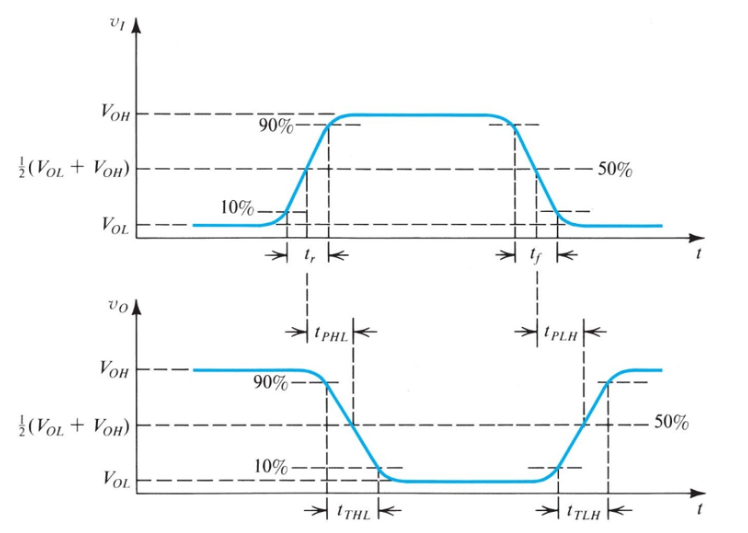
\includegraphics[width=0.6\textwidth]{tphl.png}
    \caption{Illustration of propagation delay and transition time of a logic gate. \cite{Sedra/Smith}}
    \label{fig:tphl}
\end{figure}

Figure \ref{fig:tphl} shows the different timing parameters for a logic gate. The propagation delay high-to-low $t_{pHL}$ and propagation delay low-to-high $t_{pLH}$ are the time it takes for the output to switch as input switches, measured from 50\% of the input signal to 50\% of the output signal. The rise time $t_{r}$ is the time it takes during transition for the output to switch from 10\% to 90\% of maximum output voltage. The fall time $t_{f}$ is the time it takes for the output to switch from 90\% to 10\% of maximum output voltage.

\subsection{RC circuit model of CMOS inverter}
The switching behavior of a CMOS inverter could be modeled as an first order RC network where the input capacitance of the inverter $C_I$ is charged or discharged through the resistive elements. The system can then be described by the time constant $\tau$ of the model circuit, given by the product of the resistance and the capacitance as given in the lab manual:
\begin{equation}\label{eq:tau} \tau = R_{on}C_{tot}\end{equation}
 where $R_{on}$ is resistive model for a transistor and $C_{tot}$ is the load capacitance.

\subsection{Miller effect}
The Miller effect refers to the phenomenon which describes the increase in effective capacitance between the input and output terminals of an active device due to feedback at the point of amplification. In essence, it refers to the phenomenon where a input capacitance is magnified as a result of the voltage gain of the circuit, leading to an apparent increase in input capacitance during signal transitions. This effect has implications for the design and performance analysis of amplifiers, as well as digital circuits such as CMOS inverters.

\paragraph{} In the context of the latter, the Miller effect is especially pronunced during the transition of signal levels, specifically at the switching point $V_{dd}/2$. During this critical switching point, the output capacitance effectively gets coupled back to the input through the inverter's feedback mechanism. As a result, a momentary surge in effective capacitance is experienced, the Miller capacitance, coinciding with the maximum voltage gain of the inverter.


\section{Materials and Methods}
\subsection{Equipment}
\begin{table}[h!]
    \centering
    \begin{tabular}{|c|c|c|}
        \hline
        \textbf{Component} & \textbf{Model} & \textbf{Quantity} \\
        \hline
        Resistor & 100k$\Omega$ & 1 \\
        Hex Inverter IC & 74HCT14 & 1 \\
        Copper wires & - & 12 \\
        Printed Circuit Board & - & 1 \\
        Soldering iron & - & 1 \\
        Soldering wire & - & 1 \\
        Oscilloscope & HP54622 & 1 \\
        Waveform generator  & HP33120 & 1 \\
        Voltage source & HPE3631 & 1 \\ 
        \hline
    \end{tabular}
    \caption{List of components used in the experiment.}
    \label{tab:bom}
\end{table}

\subsection{Task 1a}

\begin{figure}[h!]
    \centering
    \begin{subfigure}{.5\textwidth}
      \centering
      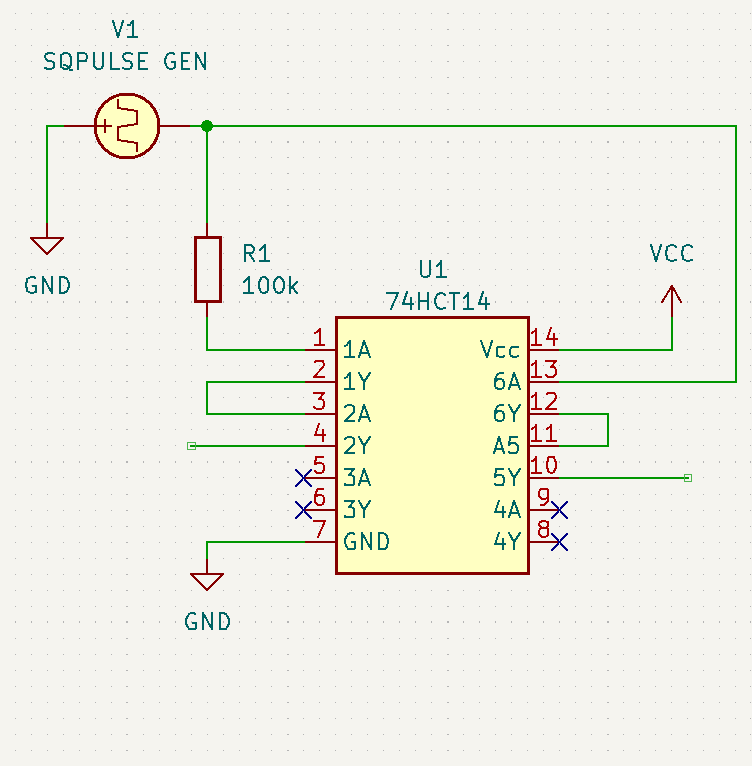
\includegraphics[width=.78\linewidth]{Task 1 Circuit.png}
      \caption{Circuit diagram}
      \label{fig:sub1}
    \end{subfigure}%
    \begin{subfigure}{.5\textwidth}
      \centering
      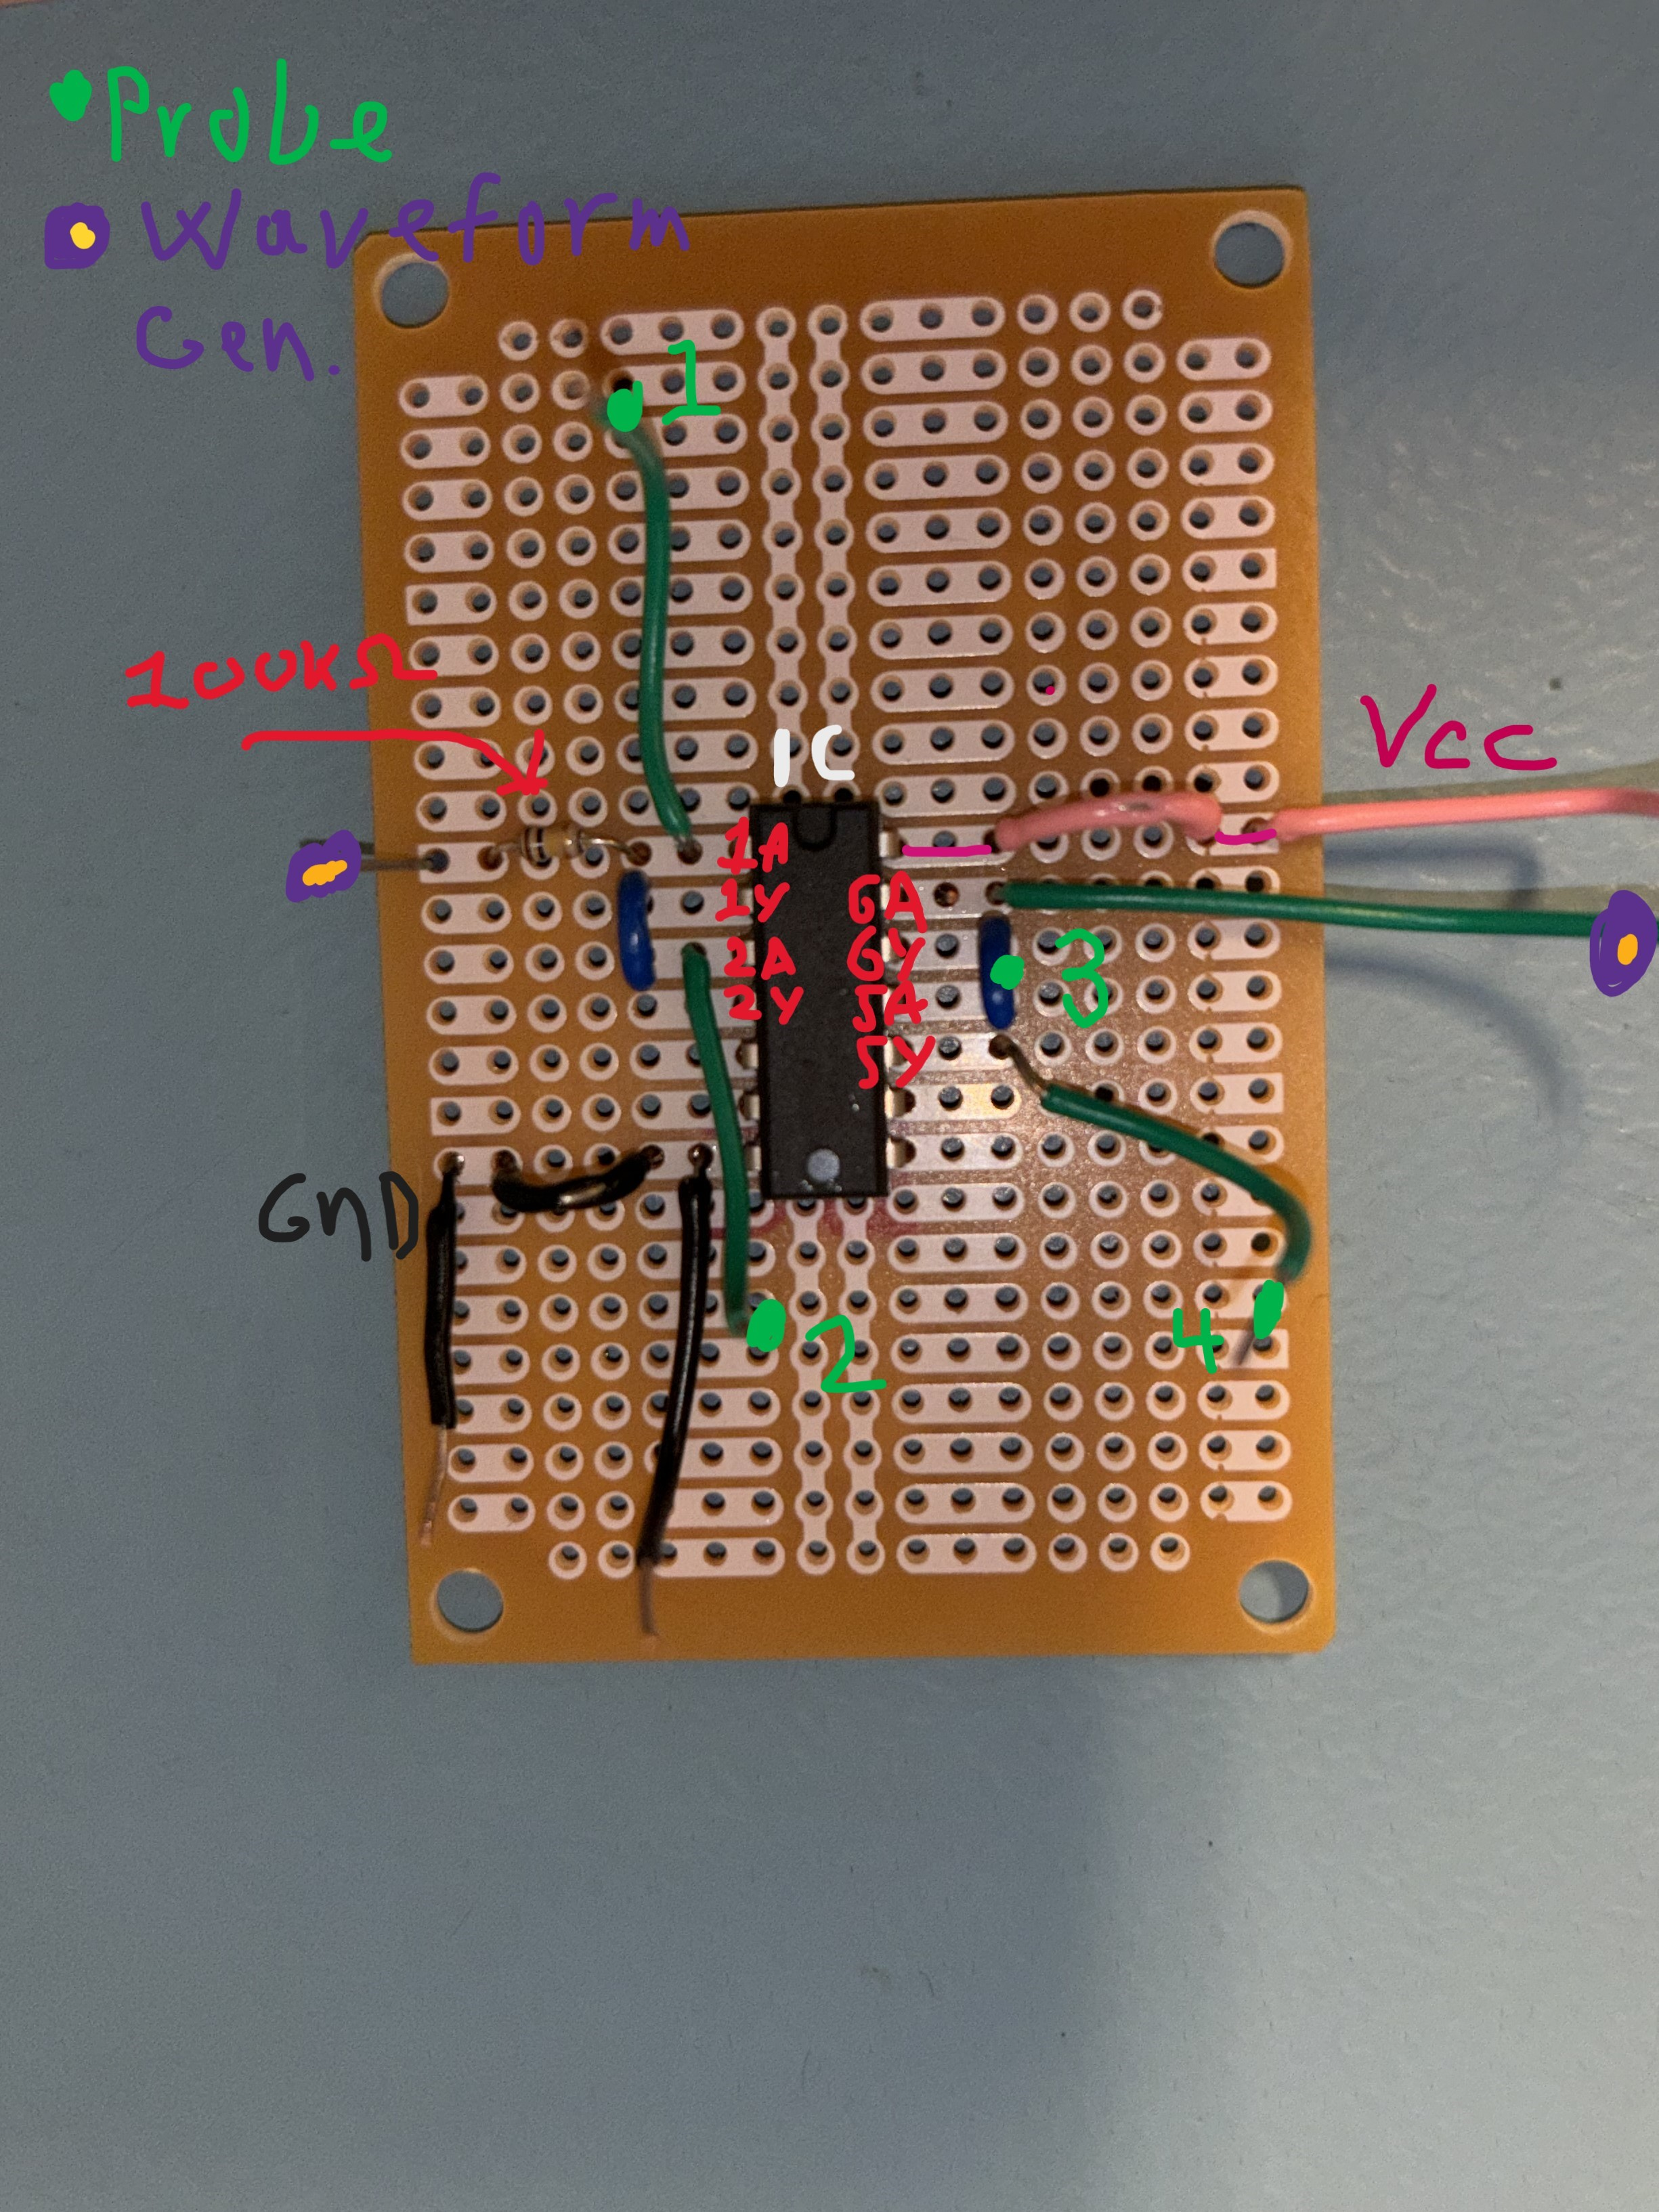
\includegraphics[width=.6\linewidth]{Photo of circuit 2.jpg}
      \caption{Photo of the circuit}
      \label{fig:sub2}
    \end{subfigure}
    \caption{Schematic and photo of two double inverters connected in series}
    \label{fig:1}
\end{figure}

The GPIB instruments are set up according to the lab manual.
The circuit is built according to the schematic in Figure \ref{fig:sub1}. The circuit has two separate serial double inverters, one with a 100k$\Omega$ resistor before the first inverter, and one without a resistor. The circuit is powered by a voltage source with a voltage of 5V. The probes of the circuit is connected to an oscilloscope in order to measure the voltage. The input marked 1A of the IC is connected to a waveform generator which generates a square wave with a frequency of 400 Hz. The circuit is then probed according to Figure 1 in the lab manual (point 1 in figure \ref{fig:sub2}).

Together with the lab manual there is supplied a Matlab script that controlls the settings of the waveform generator and the voltage source. It also reads the data from the oscilloscope and plots the data. From the given Matlab script the following modification were made:
\begin{itemize}
  \item The waveform generator was set to generate a square wave with a frequency of 400 Hz and peak voltage of 5 V on line 35 and 36.
  \item Autoscale for the oscilloscope was disabled on line 40.
  \item A system-specific dc offset was added to the oscilloscope to keep the signal within the 0 - 5 V range.
  \item The for-loop between lines 64 - 69 was swapped for a single line that set the voltage source to a constant 5V.
  \item All plotting were modified to be labeled with correct axes and title.
\end{itemize}

In order to capture a single low-to-high transition, the oscilloscope display were manually adjusted as needed.

From the plotted data, the start point, end point of the rising edge and the switching point at $V_{dd}/2$ were marked. These were then used to find the input capacitance of the inverter using equation \ref{eq:tau}.

\subsection{Task 1b}
The wavegenerator is connected to input 6A of the IC. The probe measures the signal at point 3 from figure \ref{fig:sub2}. Another probe measures the output of the second inverter at point 4 from figure \ref{fig:sub2}. The settings on the instruments are kept the same as in task 1a. The Matlab script is modified to plot the data from both channels from the oscilioscope. The script is then run to capture the high-to-low and low-to-high transitions of the circuit, which were found by manually adjusting the oscilloscope display.

\clearpage

\section{Results}
\subsection{Task 1}
\textbf{Plot of the rising edge of a double inverter circuit with a 100k$\Omega$ resistor before the first inverter:}
\begin{figure}[h!]
  \centering
  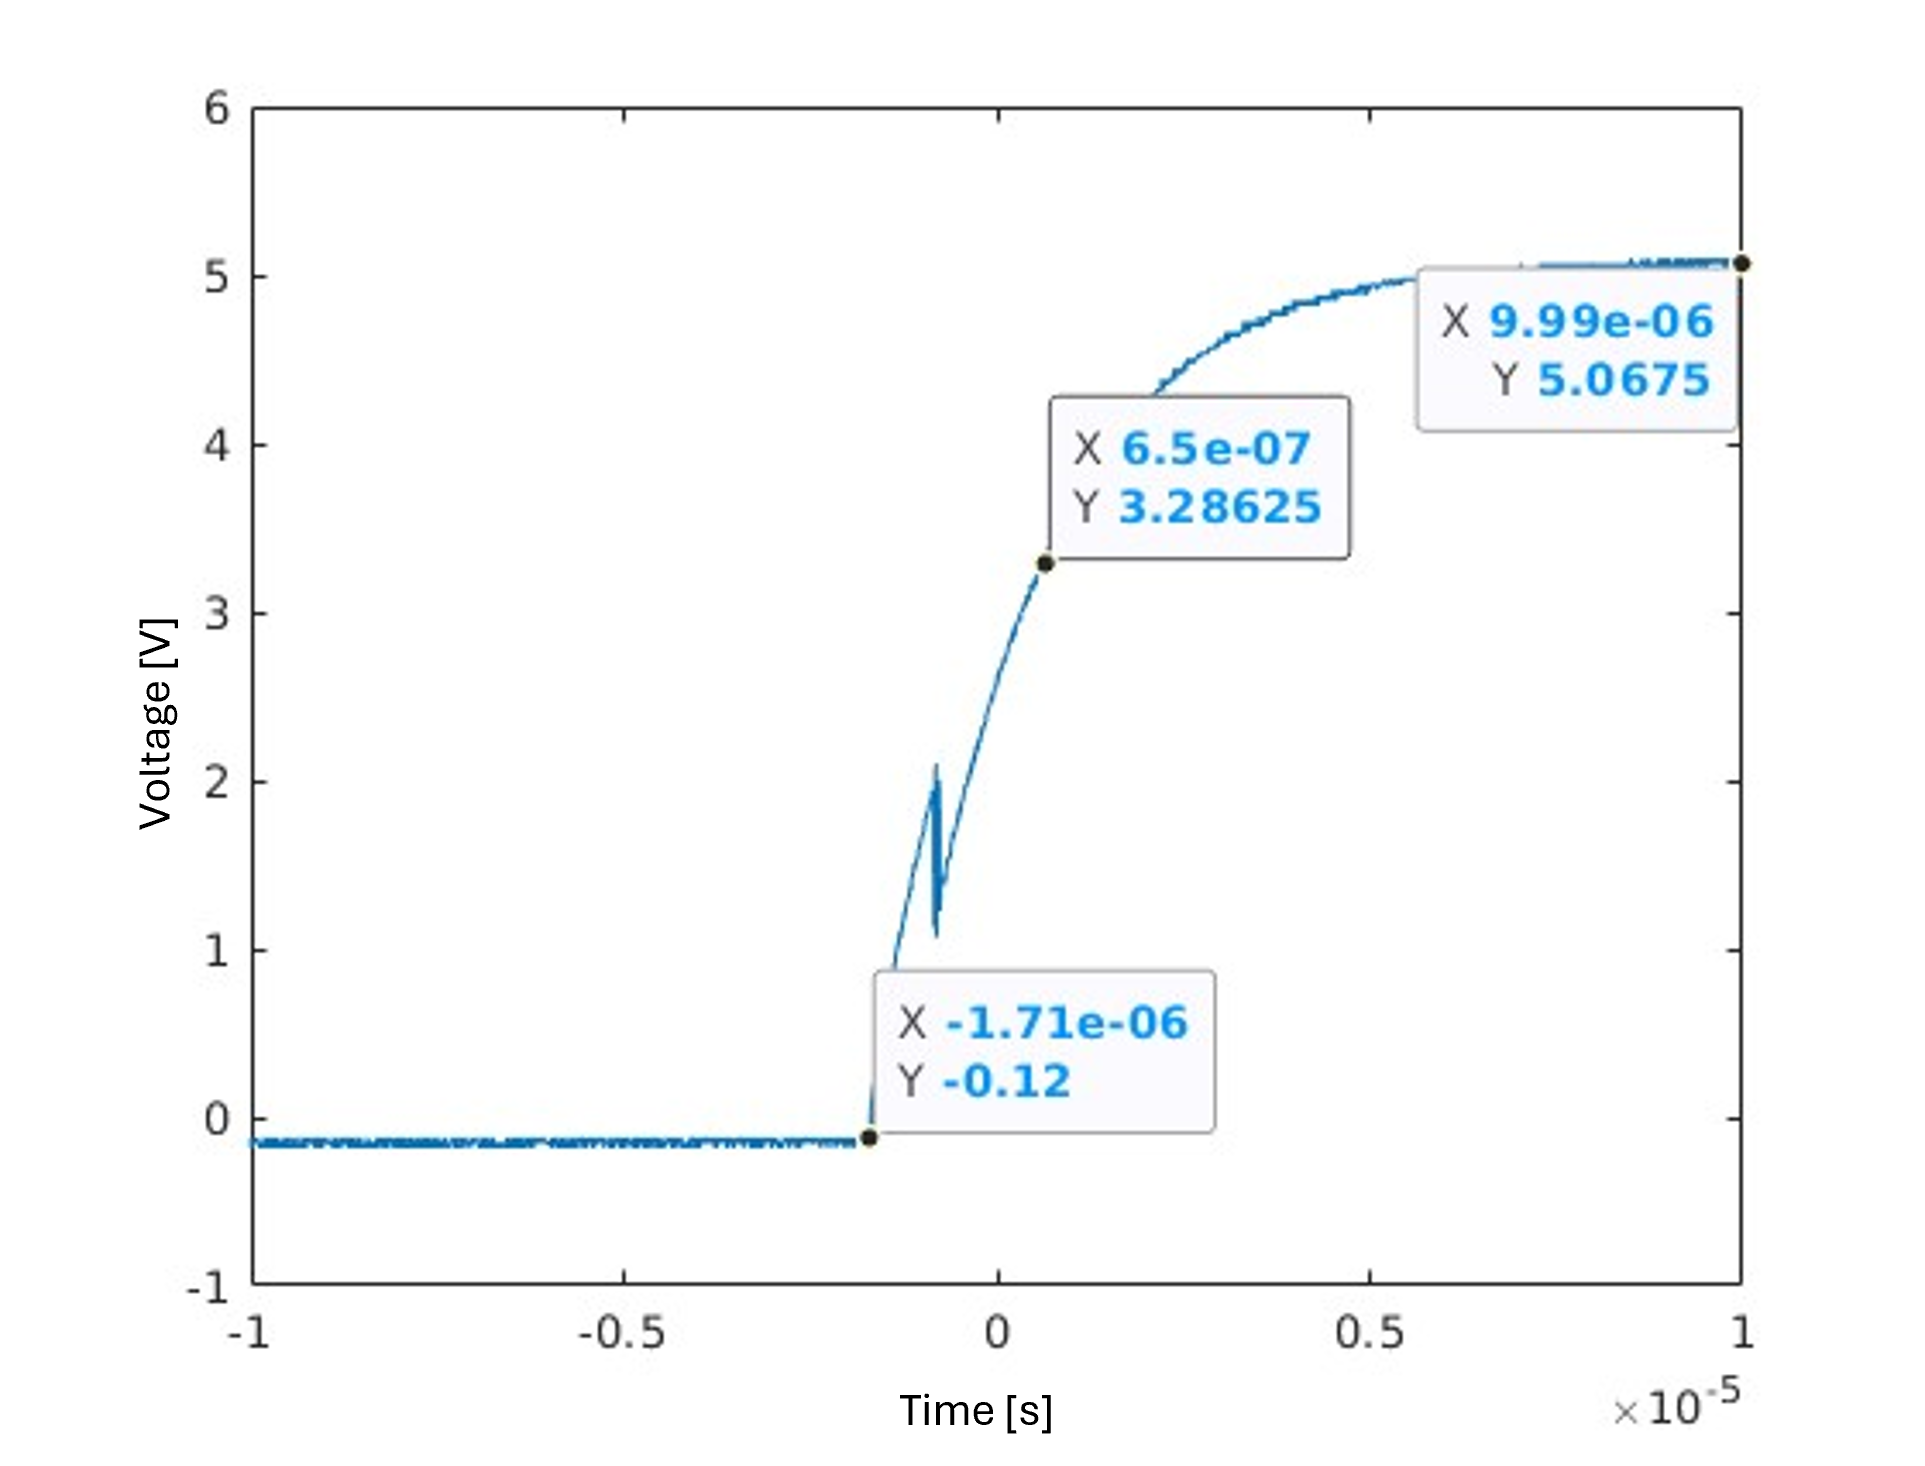
\includegraphics[width=0.6\textwidth]{plot1.png}
  \caption{Plot of the rising edge of a double inverter circuit with a 100k$\Omega$ resistor before the first inverter with added points of interest.}
  \label{fig:plot}
\end{figure}

\textbf{Plot of the edges of a double inverter circuit without a resistor before the first inverter:}

\begin{figure}[h!]
  \centering
  \begin{subfigure}{.5\textwidth}
    \centering
    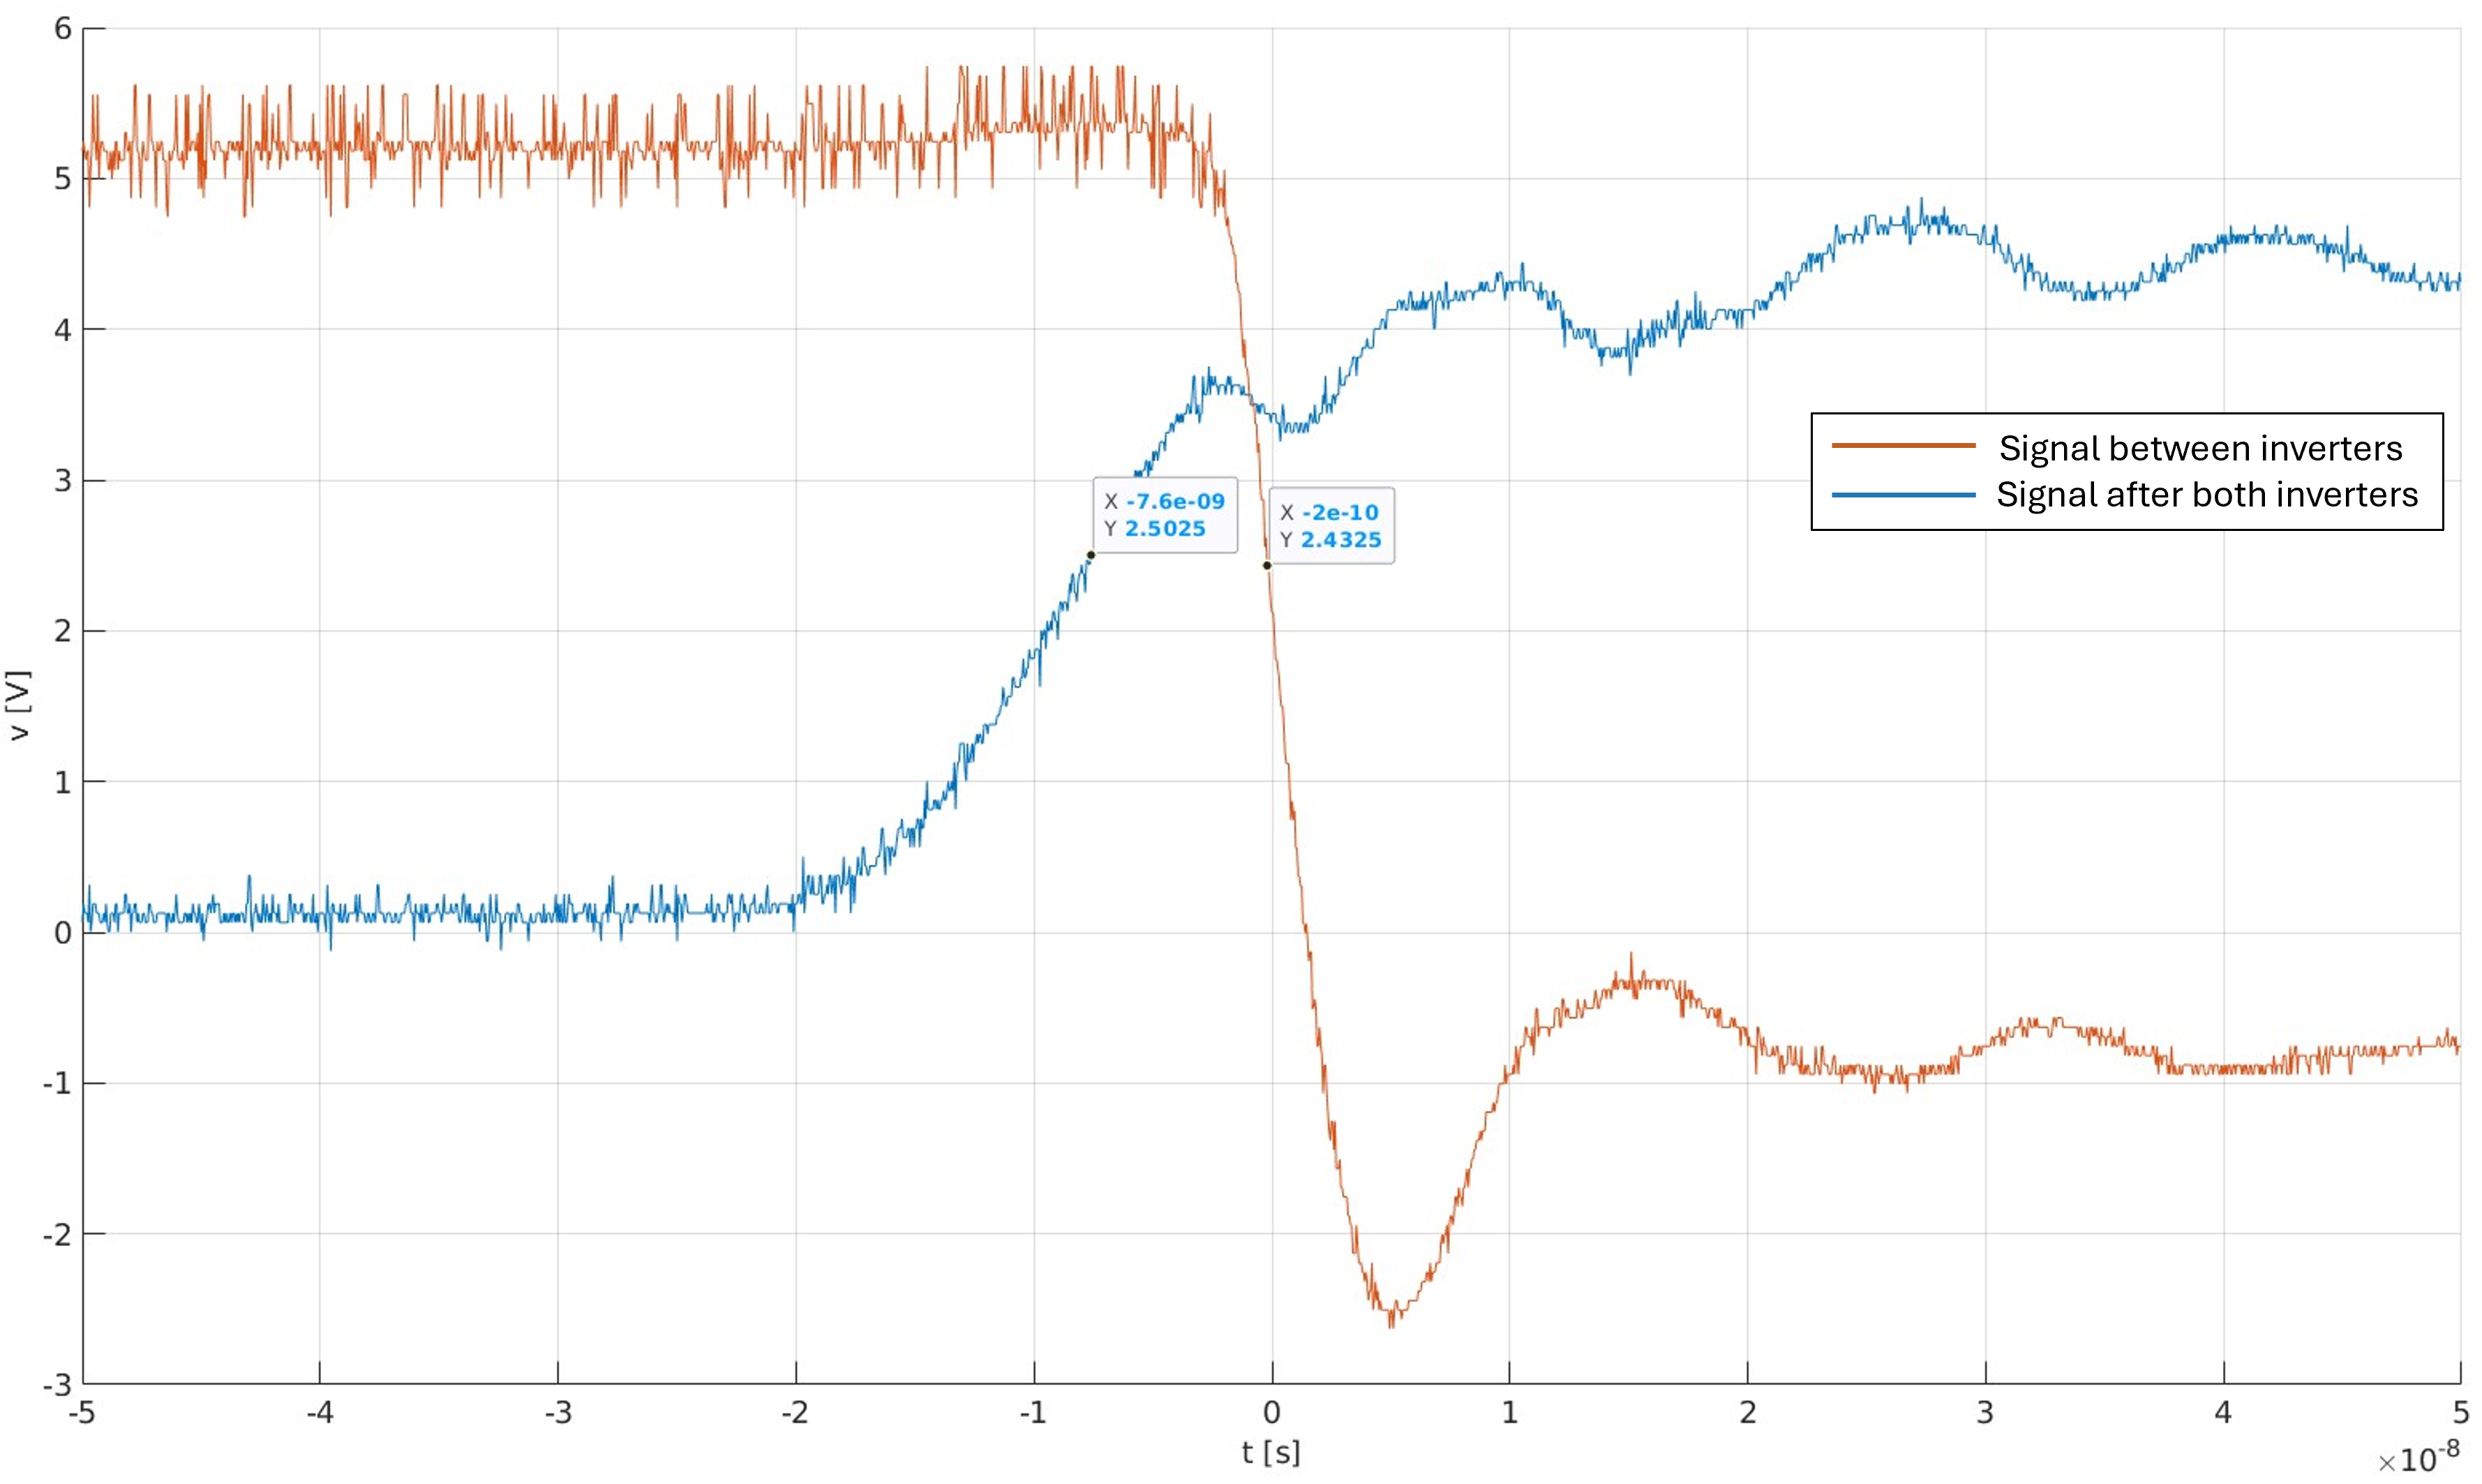
\includegraphics[width=.8\linewidth]{task2bhl2.png}
    \caption{High-to-low transition}
    \label{fig:sub3}
  \end{subfigure}%
  \begin{subfigure}{.5\textwidth}
    \centering
    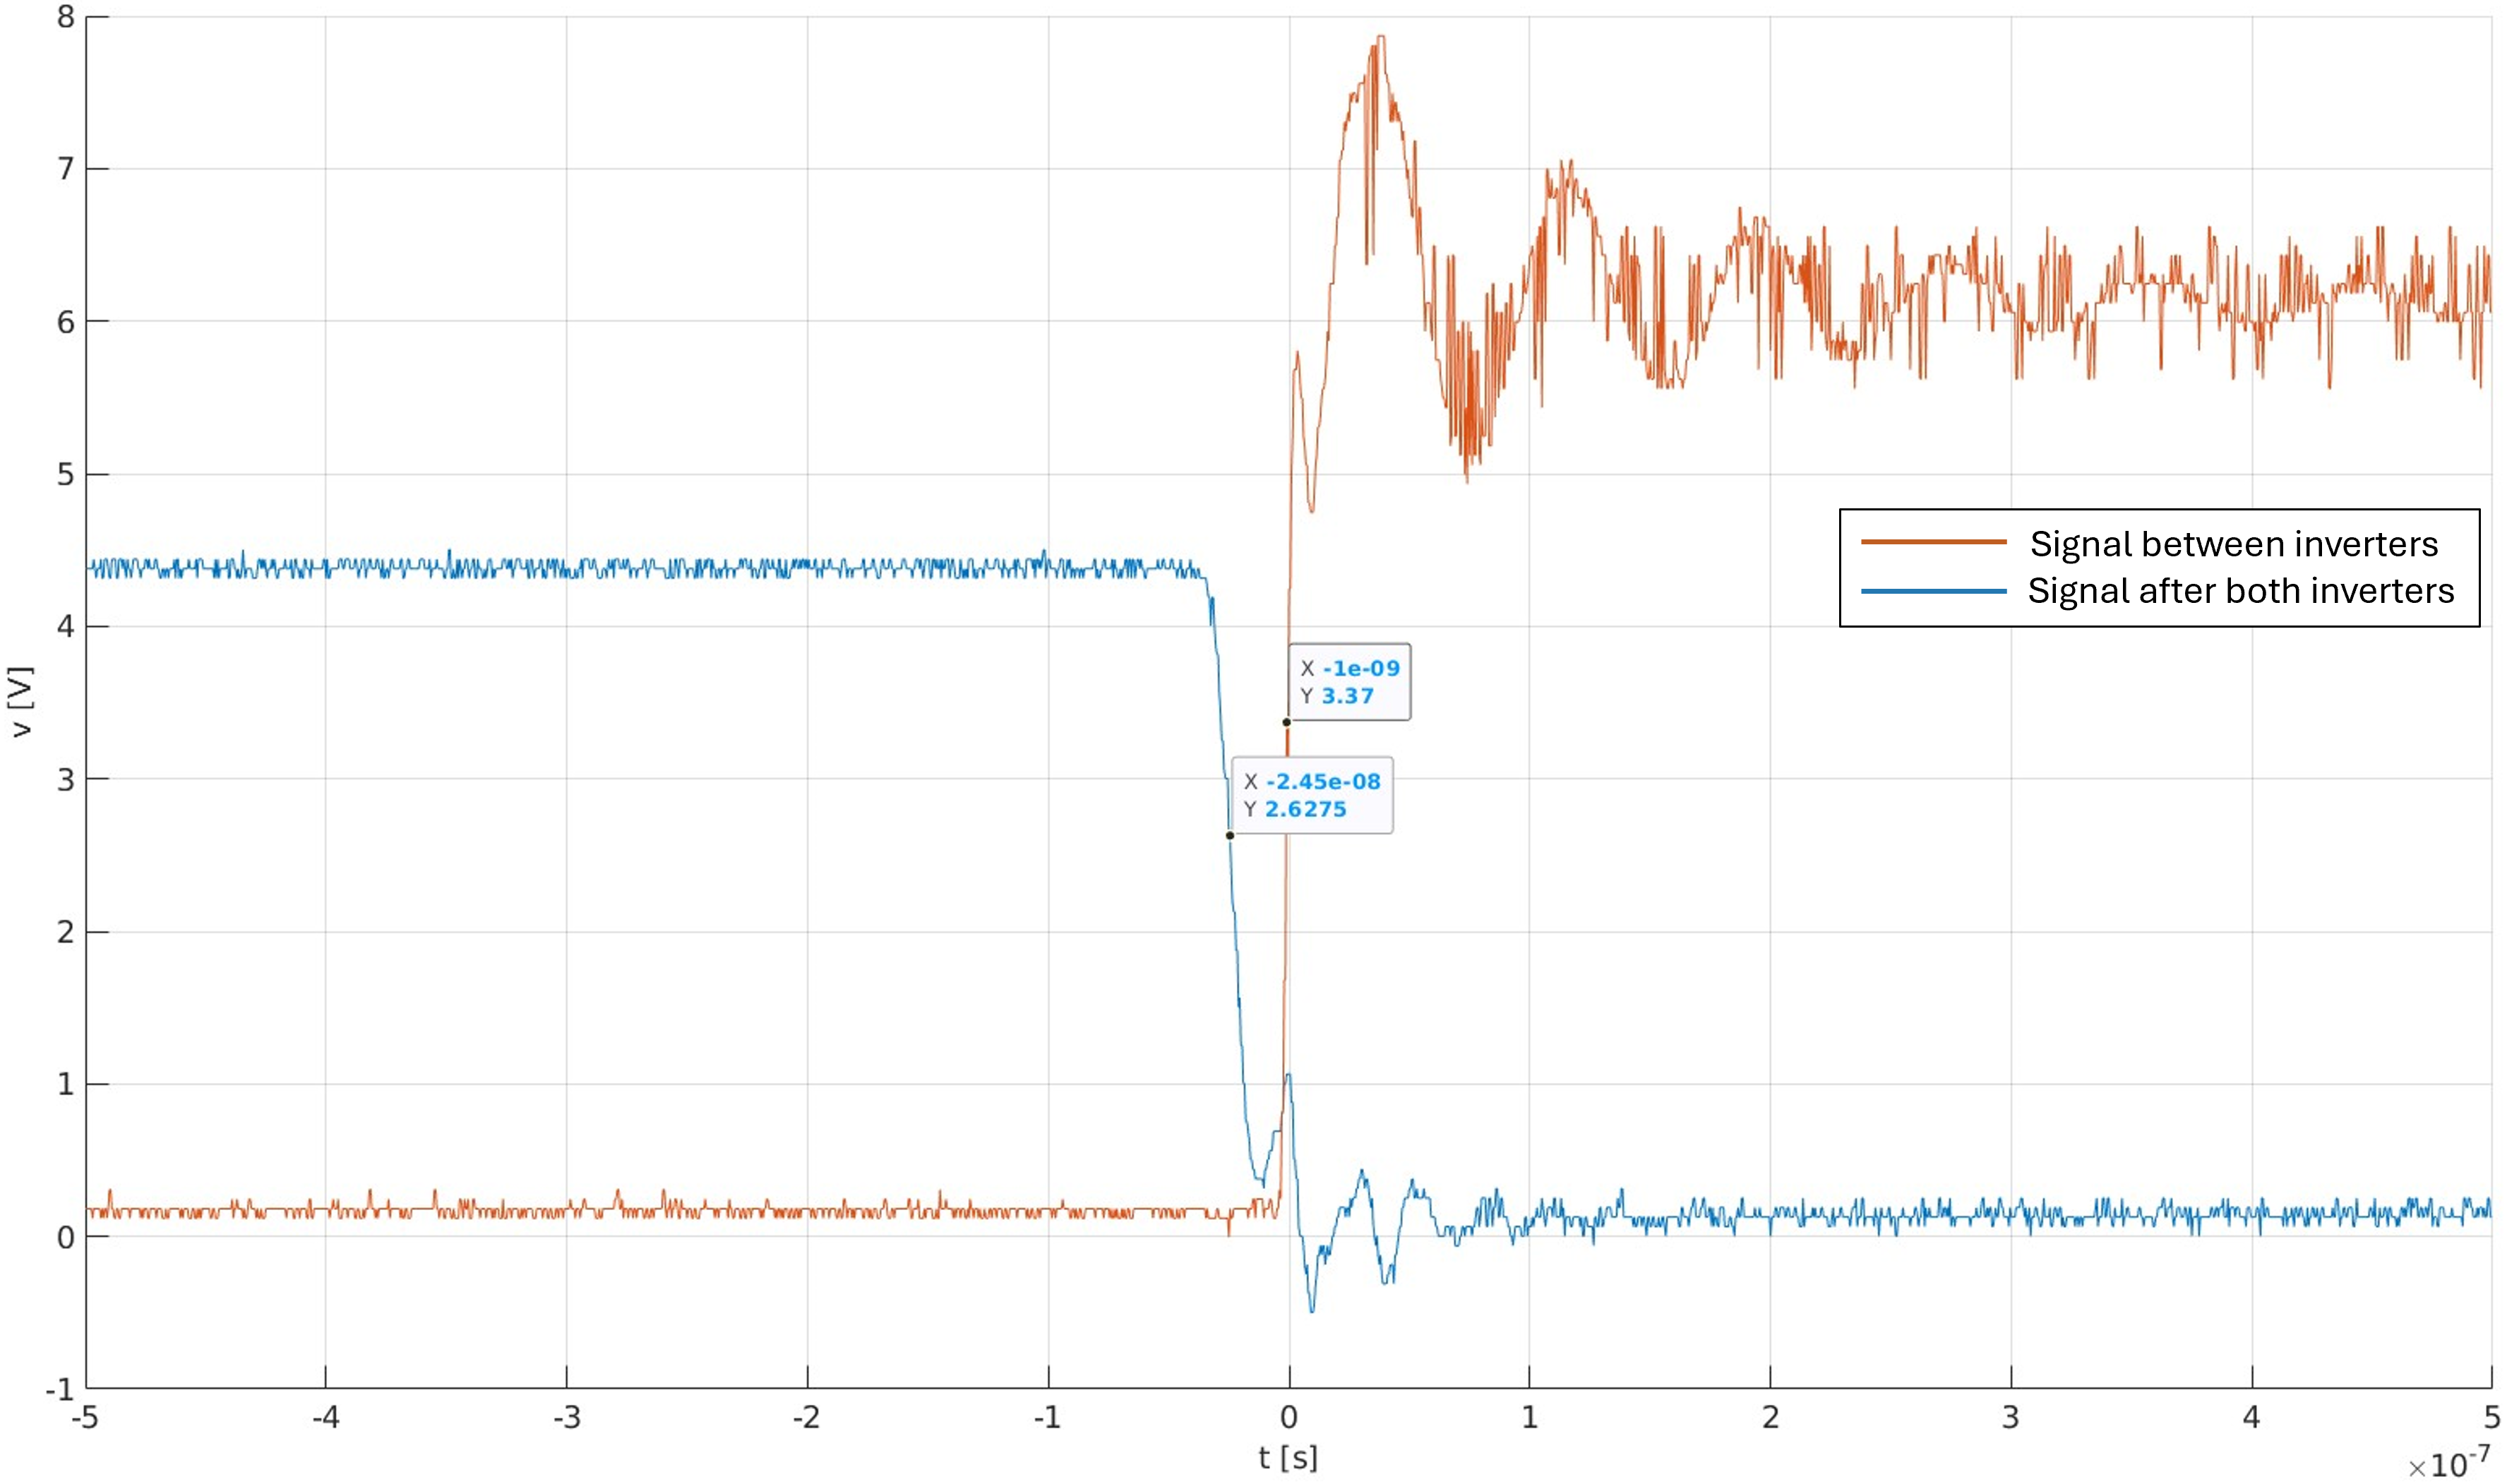
\includegraphics[width=.8\linewidth]{task2blh2.png}
    \caption{Low-to-high transition}
    \label{fig:sub4}
  \end{subfigure}
  \caption{Plots of the edges of a double inverter circuit without a resistor before the first inverter.}
  \label{fig:2}
\end{figure}

\paragraph{Input capacitance of the inverter:}
\begin{equation}
    C_{I} = 8.6 \ \text{pF}
\end{equation}


\section{Discussion}

\subsection{Inaccuracy in measurements}
\paragraph{Task 1a:} 
When measuring capacitances in a circuit, it is important to remain aware of several factors that could introduce errors in the measurements. The length of the copper wires, the quality of the soldering, components, and instruments may introduce noise or other parasitic capacitance that alter the measurements. In this experiment, all potential factors have been neglected, with the excepetion of the oscilloscope probe capacitance which was subtracted from the total capacitance as in accordance with the lab manual.

\paragraph{Task 1b:} In figure \ref{fig:2} there are considerable amount of noise distorting the signal. This is especially noticable in the high-regions of the signal between inverters. Investigation into the cause of this noise considered the oscilloscope probe, the oscilloscope itself and the grounding of the circuit as potential sources of error. The circuit was also replicated once on a new PCB, and also once on a breadboard, but the noise persisted. Changing instruments and cables had little to no effect either. After several attempts to fix the problem and extensive time spent troubleshooting, it was decided, together with the lab supervisor, the noise made it not possible to accurately calculate $\tau_{LH}$, $\tau_{HL}$, $R_{ONp}$, and $R_{ONn}$. 

\paragraph{} As $V_{dd}$ is set to 5 V the expected range of voltages for the input and output signals are 0 - 5 V. In figures \ref{fig:plot} and \ref{fig:2} the signals can go both over and under the range. Sources of error discussed in the two above paragraphs could be the cause of this. For task 1A, the points of interest are marked on the graph by method of 'eyeballing', which can cause some inaccuracies in the measurements. The sample rate used to generate the plot is also limiting in how close the points can be marked. All these factors can contribute to the inaccuracy of the measurements and further calculations. 
\subsection{Repercussions of the Miller effect}
In figure \ref{fig:plot} there is a noticable notch in the transition from low-to-high. This kickback on the input happens at the switching point $V_{dd}/2$ in transition and is due to the Miller effect feedback. As propagation delay is defined to be the time difference between the input and output signal at 50\% of the transition, and the miller effect does not eject charge back before the voltage exactly reaches the switching point, the effect is not relevant for the calculations.

\section{Appendix}
\subsection{Calculations}
\paragraph{Input capacitance of the inverter:}
From equation \ref{eq:tau} we use algebra to solve for $C_{I}$ with values from figure \ref{fig:plot}:
\begin{align}
    \tau &= R_{on}C_{tot} \nonumber \\
    \Rightarrow C_{tot} &= \frac{\tau}{R_{on}} \nonumber \\
    C_{I} + 15 \ \text{pF} &= \frac{\tau}{R_{on}} \nonumber \\
    C_{I} &= \frac{(6.5\cdot 10^{-7} \ \text{s}) - (-1.71 \cdot 10^{-6} \ \text{s})}{100 \ \text{k}\Omega} - 15 \ \text{pF}\nonumber \\
    C_{I} &= 8.6 \ \text{pF} \nonumber
\end{align}
Note: The lab manual states that 15 pF is to be subtracted from the total capacitance to get the input capacitance of the inverter. This is done to account for the capacitance of the oscilloscope probe.

\begin{thebibliography}{9}
\bibitem{Kompendium} Philipp Häfliger. (2024). \textit{Microelectronics Essentials} (beta 0.10). Department of Informatics, University of Oslo.
\bibitem{Sedra/Smith} Philipp Häfliger (2018). \textit{Excerpt of Sedra/Smith Chapter 15: Inverter Delay} [PDF].  Department of Informatics, University of Oslo. \url{https://www.uio.no/studier/emner/matnat/ifi/INF3410/h18/forelesningsfoiler/chapter15.pdf}
\bibitem{Neureuther} Neureuther, A.R. (2001). Lecture 24: CMOS Capacitance and Circuit Delay [PDF]. University of California, Berkeley. \url{https://inst.eecs.berkeley.edu/~ee42/fa01/LectNotes/42_24.pdf}
\end{thebibliography}
\end{document}